% ============================================================
%  2N3904 (TO-92) physical pinout - front view.
%  Hold the transistor with the FLAT FACE toward you and the
%  LEGS POINTING DOWN. Left to right the pins are E, B, C.
%  Compile:  pdflatex pinout.tex
% ============================================================
\documentclass[border=12pt]{standalone}
\usepackage{tikz}
\usetikzlibrary{calc}

\begin{document}
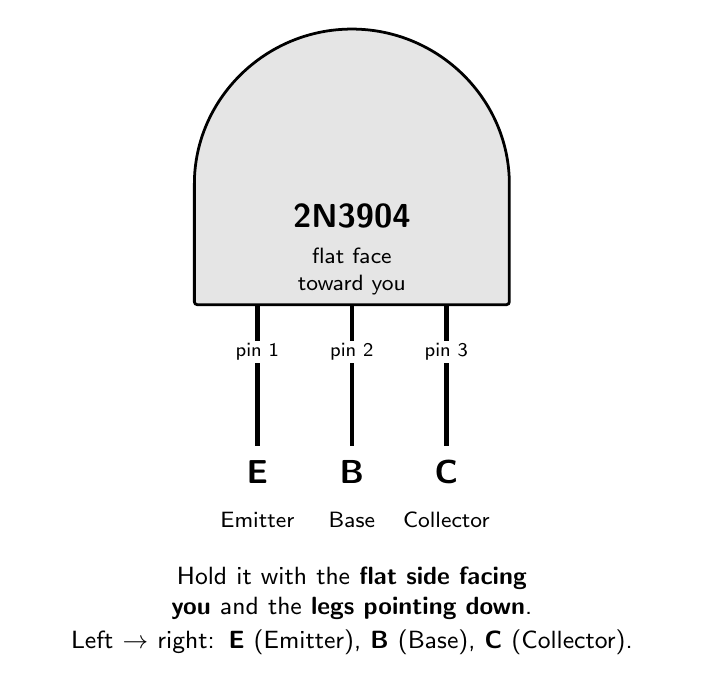
\begin{tikzpicture}[line width=1pt, font=\sffamily]

  \def\w{2.0}   % body half-width
  \def\h{1.5}   % body straight-side height

  % ---- body: flat bottom, rounded top (TO-92 seen from the front) ----
  \draw[fill=black!10, rounded corners=1pt]
        (-\w,0) -- (-\w,\h) arc (180:0:\w) -- (\w,0) -- cycle;
  \node at (0,\h*0.75) {\textbf{\large 2N3904}};
  \node[align=center] at (0,\h*0.28) {\footnotesize flat face\\[-2pt]\footnotesize toward you};

  % ---- legs ----
  \foreach \x/\lab/\full in {-1.2/E/Emitter, 0/B/Base, 1.2/C/Collector}{
     \draw[line width=1.6pt] (\x,0) -- (\x,-1.8);
     \node[below] at (\x,-1.85) {\textbf{\large \lab}};
     \node[below] at (\x,-2.5) {\footnotesize \full};
  }

  % ---- pin numbers ----
  \foreach \x/\n in {-1.2/1, 0/2, 1.2/3}{ \node[fill=white,inner sep=1pt] at (\x,-0.6) {\scriptsize pin \n}; }

  % ---- caption ----
  \node[below, align=center, text width=8cm] at (0,-3.2)
     {\small Hold it with the \textbf{flat side facing you} and the
      \textbf{legs pointing down}.\\
      Left $\rightarrow$ right: \textbf{E} (Emitter), \textbf{B} (Base), \textbf{C} (Collector).};

\end{tikzpicture}
\end{document}
